\section{Automatische Partitionierung}Bei der automatischen Partitionierung werden alle Daten auf der Festplatte gel�scht und zwei neue Partitionen angelegt. Es wird eine Partition f�r Daten und das Betriebssystem und die andere zum tempor�ren Auslagern (Swappen) erstellt.\\
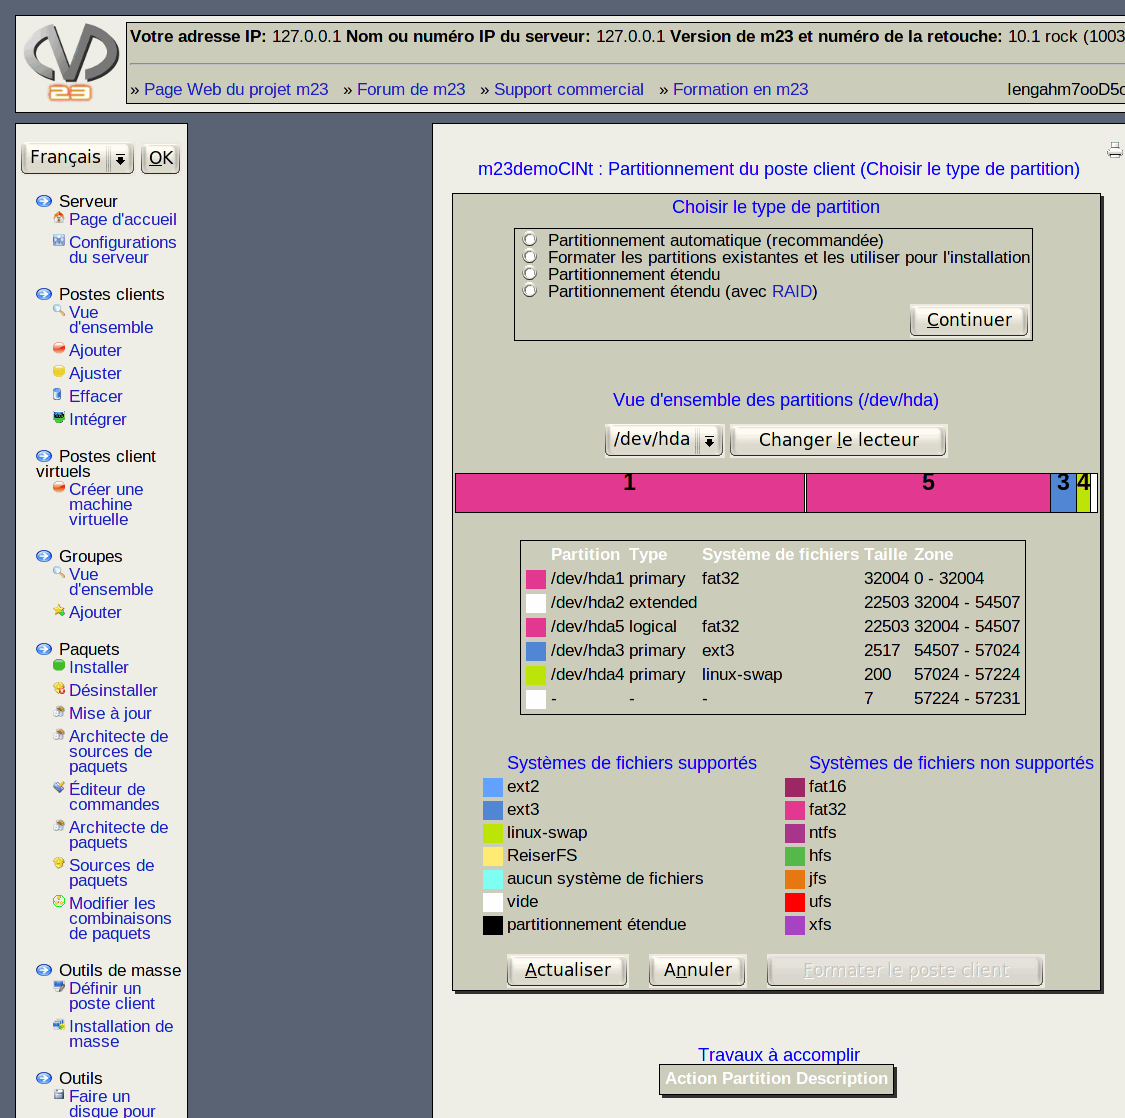
\includegraphics[scale=0.4]{/mdk/doc/manual/screenshots/de/fdisk-automatic.png} \\
\subsection{Schrittweises Vorgehen:}
\begin{enumerate}
\item W�hlen Sie \textit{"Automatische Partitionierung"}.\\
\item Durch Klicken des \textit{"Aktualisieren"}-Buttons k�nnen Sie die vorgeschlagene Partitionierung begutachten.\\
\item Klicken Sie auf \textit{"Client formatieren"}, um die Angaben zu �bernehmen.\\
\end{enumerate}
